\documentclass[11pt]{article}
\usepackage[review]{acl}
\usepackage{times}
\usepackage{latexsym}
\usepackage{booktabs}
\usepackage{graphicx}
\usepackage{amsmath}
\usepackage{multirow}
\usepackage{url}

\newcommand{\bb}[1]{\textbf{#1}}

\title{How Should Urdu Documents Be Chunked for Retrieval?\\
A Budget-Matched Study of Chunk Size, Overlap, Sentence Boundaries and Tokenization}

\author{Anonymous ACL submission}

\begin{document}
\nolinenumbers
\maketitle

\begin{abstract}
Retrieval systems are shaped by how documents are cut into chunks. Most of what we know about
that choice comes from English, and most of it measures size in model tokens. This paper moves the
question to Urdu. We build a parallel Urdu--English corpus from UQA and SQuAD2.0: 150 articles and
7{,}362 test questions. Four multilingual encoders, BM25, and BM25+dense RRF run over five chunkers,
word sizes from 50 to 800 (10 to 800 for a bge-m3 extension), token budgets from 64 to 256, and
three overlap levels. Budget-matched recall at 500 words is the metric; intervals come from an
article-level bootstrap. Three results stand out. The best tested word size is 50 for every encoder
in the main grid; extending bge-m3 down to 10 words is monotonic and also selects 50. At 10 words,
18.2\% of answers are split across chunks, against 4.1\% at 50. The token argmax differs
(64/128/256), though adjacent
budgets are statistically tied;
128 tokens is about 96 words for XLM-R and 42 for Qwen3 (fertility 1.34 vs.\ 3.07). Urdu-aware
sentence splitting beats English-toolkit defaults by 5.5--6.9 points at 50 words in the four systems
where both were run; at 200 words the sign flips. 25\% overlap is associated with 2.6--7.2 more
points on this corpus in the four systems where it was run, whereas the English studies we reviewed
found neutral or negative effects, while orthographic normalization changes nothing measurable on
this machine-translated corpus. English is easier on the parallel control but
has the same best tested fixed-word size. Code, configurations, and per-question metrics are
available at the \href{https://github.com/devxyasir/urdu-chunking-strategy}{public repository}.
\end{abstract}

\section{Introduction}

Urdu has more than 230 million speakers. Retrieval research has not kept up. Mr.\ TyDi covers
eleven languages \citep{zhang2021mr}, MIRACL eighteen \citep{zhang2022making}, mMARCO thirteen
\citep{bonifacio2021mmarco}; Urdu appears in none of them. The resources that do exist are recent:
UQA \citep{arif2024uqa}, Urdu MS MARCO \citep{butt2024enabling}, and a small cluster of papers on
alignment and Urdu question answering \citep{faheem-etal-2026-beyond,ahmad-etal-2026-drrag}. None of
them varies how documents are segmented.

Segmentation decides what a retriever can return. English work shows the stakes: size sweeps move
recall \citep{bhat2025rethinking,bennani2026a,wang2024searching}, semantic chunking rarely earns its
cost \citep{qu2024is}, and structure-aware segmenters help in some settings
\citep{yepes2024financial,singh2026parser}. Two questions remain open.

The first is the unit. Nearly every study sizes chunks in model tokens. Tokenizers do not treat
languages alike \citep{petrov2023language,ahia2023do,srivastava2026the}. For Urdu the gap is wide:
the XLM-R tokenizer behind bge-m3 and multilingual-e5 emits 1.34 tokens per word; Qwen3 emits 3.07.
A 256-token chunk is roughly 192 words for one family and 83 for the other. If the optimum is stable
in words but not in tokens, specify words. If it is stable in neither, tune per model.

The second question is whether English-toolkit defaults travel. Recursive splitters reach for blank
lines, line breaks, spaces, and the ASCII period. Urdu ends sentences with U+06D4 and questions with
U+061F; its orthography tolerates Arabic/Persian letter variants, zero-width joiners, and optional
diacritics. A language-aware chunker built for Khmer, the only one we found, did worse than plain
recursive splitting \citep{chhoun2026evaluation}. Whether that generalises is unknown.

We ask four questions. (Q1) How do size, overlap, and strategy interact with the retriever family
(BM25, dense, hybrid)? (Q2) Is the best size stable in words rather than model tokens across
tokenizers? (Q3) Do Urdu-aware boundaries and normalization beat English-toolkit defaults? (Q4) Does
the parallel English control select the same best tested size? The evaluation is retrieval-only: no
generator, no LLM judge. Our contributions are:
\begin{itemize}
\item a systematic, budget-matched chunking evaluation for Urdu retrieval: 360 main runs over a
  150-article pool and 7{,}362 test questions, five chunkers, four encoders, two sparse retrievers,
  and RRF, plus a four-run bge-m3 lower-size check;
\item a direct word-versus-token comparison across tokenizers with measured fertility: token budgets
  are not comparable across models, word budgets are;
\item evidence that Urdu-aware sentence splitting helps at the small sizes dense retrievers prefer
  and hurts at large sizes; 25\% overlap helps on this corpus;
\item a parallel English control on the same articles and questions, plus a null result for
  orthographic normalization on machine-translated Urdu.
\end{itemize}

\section{Related Work}

\paragraph{Chunking for retrieval.}
Fixed token windows are still the default. \citet{bhat2025rethinking} sweep 64--1024 tokens over six
English QA datasets; the optimum depends on answer type and encoder. \citet{bennani2026a} vary
50--500 tokens and 0/20\% overlap with SPLADE and a generator, and find overlap unhelpful.
\citet{wang2024searching} compare 128--2048 tokens inside a larger RAG pipeline. Semantic and
structure-aware chunkers have been compared at fixed sizes
\citep{qu2024is,zhou2026beyond,caspari2026when,merola2025reconstructing,gnther2024late}, and
granularity itself has been studied as propositions versus passages \citep{chen2023dense}. The
closest template is \citet{singh2026parser}: a factorial study of parsers, chunkers, and embedders
on English regulatory documents, analysed with mixed-effects models. We found no controlled
chunking evaluation for Urdu retrieval and no study that compares word- and token-defined sizes
across tokenizers.

\paragraph{Low-resource and multilingual retrieval.}
LaBSE \citep{feng2020languageagnostic}, multilingual E5 \citep{wang2024multilingual}, BGE-M3
\citep{chen2024m3embedding}, and Qwen3 Embedding \citep{zhang2025qwen3} all claim Urdu support;
MMTEB \citep{enevoldsen2025mmteb} covers a lot of ground. Averages mislead. On Amharic, the best
zero-shot multilingual retriever trails a monolingual model by 23\% relative MRR, and BM25 beats
four of five zero-shot dense retrievers \citep{alemneh2026the}. Hubness and cross-lingual asymmetry
distort rankings in other languages \citep{sakhawat2026hubness,goworek2025what}. Urdu work has gone
into alignment \citep{faheem-etal-2026-beyond}, dual-representation retrieval
\citep{ahmad-etal-2026-drrag}, and QA data \citep{arif2024uqa,butt2024enabling}. We found no
controlled study of Urdu segmentation for retrieval.

\paragraph{Tokenization and Urdu text.}
Tokenizers charge different prices for the same content \citep{petrov2023language,ahia2023do}, and
fertility predicts downstream accuracy in some settings \citep{lundin2025the}. Indic scripts pay a
large tax, partly structural \citep{srivastava2026the,regmi2026vowel}; single-token retention
exposes how the vocabulary is allocated \citep{nayeem2025beyond}. Urdu's literature is thinner.
CURE built an IR test collection with stemming and query expansion \citep{iqbal2020cure}; early
indexing work described normalization rules but did not test them \citep{qureshi2021an}. UQA
provides machine-translated SQuAD2.0 with preserved spans \citep{arif2024uqa}; Urdu MS MARCO
provides translated passages \citep{butt2024enabling}. We use UQA because it gives character-level
answer spans in parallel with English SQuAD2.0.

\section{Data}

\paragraph{Parallel corpus.}
We start from UQA \citep{arif2024uqa}, a machine translation of SQuAD2.0 into Urdu with preserved
answer spans, and from the original SQuAD2.0 articles. The released UQA has 124{,}745 training rows
mapped to 19{,}021 English paragraphs. One property mattered more than the rest, and we measured it
rather than assuming it: each English paragraph was translated again and again. The average
paragraph carries 4.86 distinct Urdu contexts; the maximum is 18. Pairs we inspected sit at
0.96--0.98 string similarity.

Documents are built with a \emph{modal-variant} rule. For every English paragraph we keep the most
frequent Urdu context (ties go to the longer string, then the lexicographically larger one). A
question survives only when its row uses that variant and the question is answerable. An article
document is the chosen paragraphs joined in order. Of 124{,}745 rows, 24{,}898 remain (20.0\%).
Every retained span was checked: 83{,}018/83{,}018 train and 11{,}169/11{,}169 validation rows pass
the character-offset equality test. The English control reuses the same articles and questions with
SQuAD paragraphs and offsets. On a 100-question audit with three independent raters, the majority
label is self-contained for 77, context-dependent for 21, unclear for 1, and has no majority for 1;
the self-contained rate is 77.0\% (Wilson 95\% CI 67.8--84.2\%). Pairwise raw agreement is 88--91\%,
Fleiss' kappa is 0.734, and 85/100 rows are unanimous. The audit is a corpus check, not an
evaluation of retrieval quality.

\paragraph{Pool and splits.}
We keep the 403 articles with at least 20 retained questions, 20 paragraphs, and 1{,}500 Urdu words.
They are sorted by SHA-1 of the title, and the first 150 are taken. Every fifth article is
development (30 articles); the other 120 form the test set. A question-level split would leak
chunks across the boundary, so the split is by article. Table~\ref{tab:data} gives the totals.

\begin{table}[t]
\centering
\footnotesize
\begin{tabular}{lr}
\toprule
Articles (dev/test) & 150 (30 / 120) \\
Urdu words & 1{,}007{,}122 \\
Paragraphs & 6{,}720 \\
Questions (dev/test) & 9{,}077 (1{,}715 / 7{,}362) \\
UQA variants/paragraph & 4.86 \\
Rows retained & 20.0\% \\
Span failures & 0 \\
\bottomrule
\end{tabular}
\caption{Corpus statistics. Counts are exact, not estimated.}
\label{tab:data}
\end{table}

\paragraph{Urdu boundaries and tokenization.}
Figure~\ref{fig:example} shows the linguistic contrast that drives the study: a two-sentence Urdu
passage whose word count is the same for every tokenizer but whose token count differs by
3$\times$. The study corpus holds 34{,}737 U+06D4 boundaries and only 51 U+061F question marks,
against 2{,}310 ASCII periods. Zero-width joiners are absent, tatweel appears once, and there are
nine Arabic yeh characters and 34 Urdu digits. Normalization has almost nothing to change
(Section~\ref{sec:norm}).

\begin{figure*}[t]
\centering
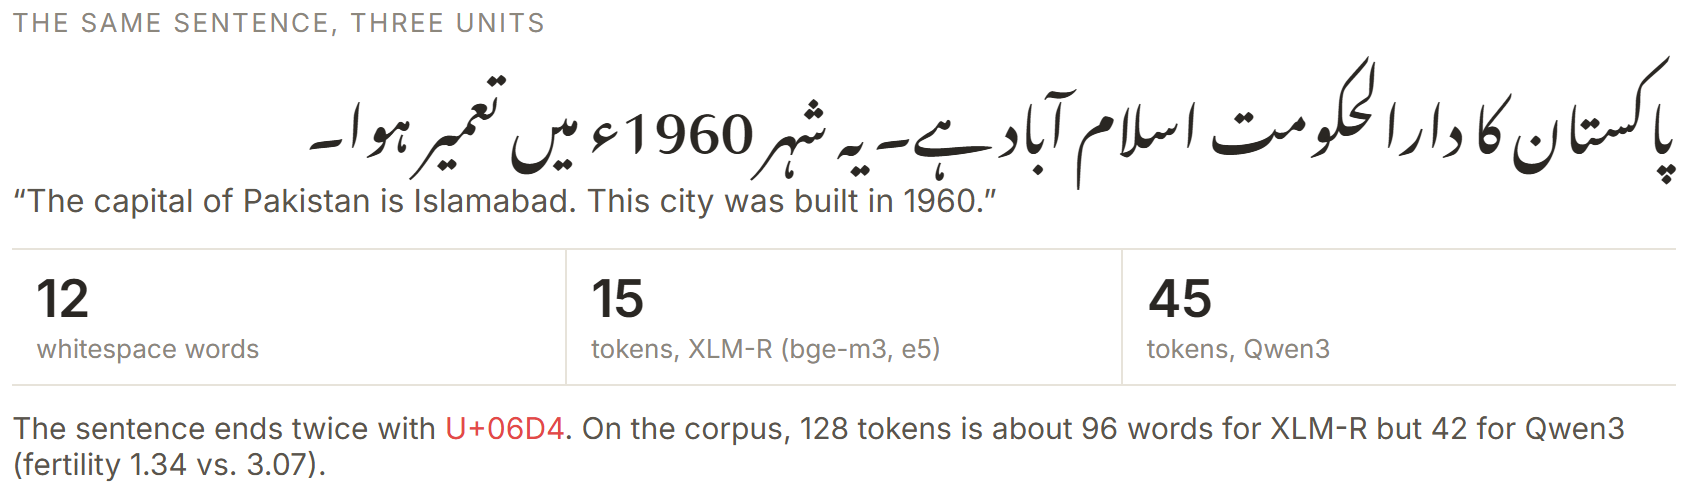
\includegraphics[width=0.95\textwidth]{urdu_example.png}
\caption{The same 12-word Urdu sentence is 15 tokens for the XLM-R tokenizer used by bge-m3 and
multilingual-e5, and 45 tokens for Qwen3. Sentence ends are U+06D4. On the corpus, 128 tokens
corresponds to about 96 words for XLM-R and 42 for Qwen3.}
\label{fig:example}
\end{figure*}

\section{Method}

\paragraph{Chunkers.}
All five chunkers return character offsets in the normalized document.
\emph{Fixed words} slides a window of $s$ whitespace words with step
$\max(1,\mathrm{round}(s(1-o)))$.
\emph{Fixed tokens} packs whole words while the model tokenizer's content-token count stays within
$b$; it steps by the same overlap fraction in words and never cuts inside a word.
\emph{Sentence-aware} splits at U+06D4, U+061F, and the exclamation mark when whitespace or a
paragraph break follows, then groups whole sentences up to a word target. Only a sentence longer
than twice the target is split by words.
\emph{Recursive-English} follows the English-toolkit separators (paragraph, newline, ASCII period
followed by whitespace and an uppercase letter or end, question mark, exclamation mark, space) and
merges units up to the target.
\emph{Recursive-Urdu} runs the same merge with Urdu terminators and paragraph breaks.
At zero overlap every chunker covers every non-whitespace character exactly once. We test that on
ten documents for every configuration: 1{,}170 checks, zero uncovered characters.

\paragraph{Retrievers.}
BM25 tokenizes on whitespace, strips Urdu and ASCII punctuation, and uses $k_1=1.2$ and $b=0.75$.
Both values were fixed in advance. BM25-char works on 3--5 character n-grams generated inside
words. Dense retrieval is cosine similarity over L2-normalized vectors from bge-m3
\citep{chen2024m3embedding}, multilingual-e5-large-instruct \citep{wang2024multilingual},
Qwen3-Embedding-0.6B \citep{zhang2025qwen3}, and LaBSE \citep{feng2020languageagnostic}. Queries use
the documented instruction formats; the same format is applied to every run. RRF fuses
BM25-whitespace and the dense ranking of the same chunk configuration with $k=60$.

\paragraph{Metrics.}
A chunk counts as relevant when it contains the full gold answer span. We report Recall@1/3/5/10,
MRR@10, nDCG@10, and the primary budget-matched recall. That last one walks the ranking, adds chunk
word counts until a budget $B$ is reached, and scores 1 if at least one retrieved chunk contains the
full answer. A span split across chunks is a failure, and we report the answer-split rate next to
recall. The primary budget is $B=500$ words; 200, 1000, and 2000 are secondary. The crossing
definition, which includes the chunk that reaches the budget, is the pre-registered one. The strict
definition appears in the appendix; it changes only the BM25 argmax. Budget-matched here means the
same 500-word query-time reading budget for every configuration. Index size, chunk count, and
embedding cost are not equalised; they are reported so the trade-off is visible.

\paragraph{Statistics.}
The analysis unit is the article, not the question. Every question in an article shares the same
chunk set, so averaging over questions would pretend to a precision the design does not have. For
each configuration we compute a per-article mean, then average over the 120 test articles.
Confidence intervals come from 10{,}000 bootstrap resamples over articles with seed 0. Paired
contrasts reuse the same resample for both configurations. The arithmetic is blunt: 61 questions share one chunk
set, and treating them as independent reports power 1.00 for a 5-point effect that the article-level
analysis detects with about 75\% power.

\paragraph{Grid.}
BM25 covers five strategies, five word sizes (50/100/200/400/800), and three overlaps (0/10/25\%).
Dense models cover 21 configurations: fixed words at 50/100/200 with 0/10/25\% overlap (9), fixed
tokens at 64/128/256 (3), and sentence-aware, recursive-English, and recursive-Urdu at 50/100/200
with zero overlap (9). bge-m3 and Qwen3 also run 400/800 words with 0/25\% overlap. LaBSE is
secondary and runs at 50/100 words. e5 stops at 200 words: its 512-token window truncates 74\% of
400-word chunks and 100\% of 800-word chunks. The encoders use their model maximum sequence lengths
(bge-m3 8{,}192, e5 512, Qwen3 32{,}768, LaBSE 256). Only LaBSE's 100-word sentence-aware run
truncates: 3 of 9{,}800 chunks (0.03\%) exceed 256 tokens; every other dense run is clean. The main
grid is 360 runs. A separate lower-size extension adds 4 bge-m3 runs at 10/25/40/50 words (overlap
0, N0), reported in \S\ref{sec:lower}.

\section{Results}
\label{sec:results}

\subsection{Size and retriever}
\label{sec:size}

Dense and sparse retrievers disagree about size (Figure~\ref{fig:size}, Table~\ref{tab:words}).
Every dense encoder does best at 50 words in the tested range and declines thereafter, with no
second peak. BM25 climbs to 200--400 words and drops at 800. At 50 words bge-m3 reaches 0.773
(95\% CI 0.758--0.789), 6.5 points above BM25's best tested 0.708 (0.688--0.729). BM25's best tested
size is four to eight times longer than the dense size.

The fall is steep. bge-m3 loses 1.6 points from 50 to 100 and 7.7 from 100 to 200; e5 loses 2.4 and
8.9; Qwen3 loses 4.7 and 8.0. Every encoder's 50--100 drop is significant (bge +1.65 [0.53, 2.80],
e5 +2.40 [1.06, 3.71], Qwen3 +4.71 [3.35, 6.11], LaBSE +5.38 [3.89, 6.86]).

\begin{figure*}[t]
\centering
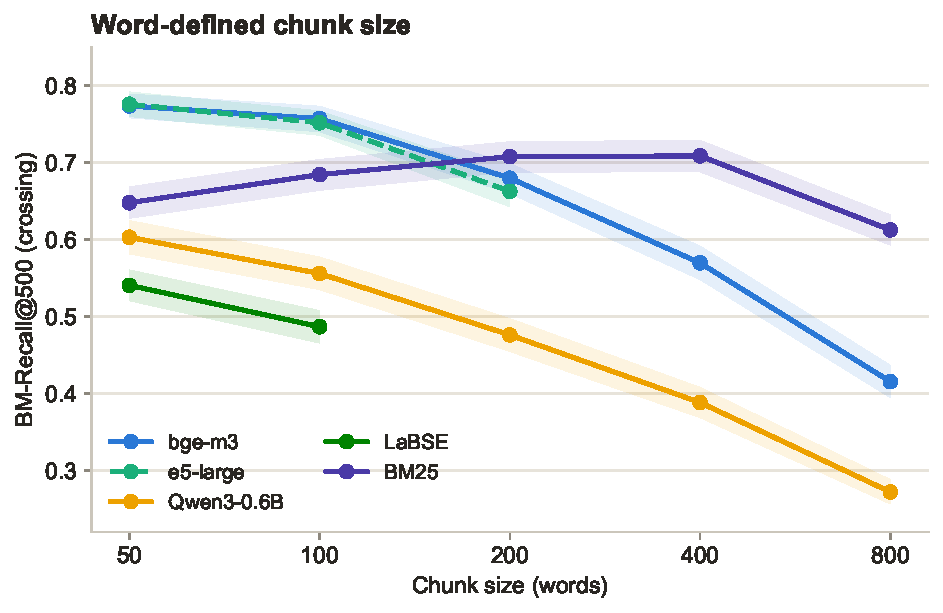
\includegraphics[width=0.86\textwidth]{../figures/fig1_word_size_curves.pdf}
\caption{BM-Recall@500 (crossing budget) against chunk size in words. Bands are 95\%
article-level bootstrap CIs. Dense encoders peak at the smallest tested size; BM25 peaks at
200--400 words. bge-m3 and e5 are nearly coincident.}
\label{fig:size}
\end{figure*}

\begin{table}[t]
\centering
\small
\begin{tabular}{lccccc}
\toprule
Model & 50 & 100 & 200 & 400 & 800 \\
\midrule
bge-m3 & \bb{.773} & .757 & .680 & .570 & .415 \\
e5-large & \bb{.776} & .752 & .663 & --- & --- \\
Qwen3-0.6B & \bb{.603} & .556 & .476 & .388 & .272 \\
LaBSE & \bb{.540} & .487 & --- & --- & --- \\
BM25 & .648 & .684 & \bb{.708} & \bb{.709} & .612 \\
\bottomrule
\end{tabular}
\caption{BM-Recall@500 by word size (overlap 0, bm500x). Bold is the row maximum; 200 and 400 are
statistically tied for BM25. Full CIs are in Figure~\ref{fig:size}.}
\label{tab:words}
\end{table}

\subsection{Lower-size check}
\label{sec:lower}

The main grid stops at 50 words for dense models. To test whether 50 is an interior maximum, we
extended bge-m3 down to 10 words on the same articles and questions (zero overlap, N0).
Table~\ref{tab:lower} reports the four runs. BM-Recall@500 rises monotonically: .418 at 10, .689 at
25, .756 at 40, and .773 at 50. The 50-word point is 1.7 points above 40, but the two intervals
overlap, so we do not claim a sharp 40-versus-50 separation. At 10 words, 18.2\% of answers are split
across chunks, against 4.1\% at 50; fragmentation is a plausible mechanism, not a decomposition.
The check
covers one encoder. e5, Qwen3, and LaBSE were not extended below 50.

\begin{table}[t]
\centering
\small
\setlength{\tabcolsep}{4pt}
\begin{tabular}{rcccc}
\toprule
Size & Chunks & BM500x [95\% CI] & BM500 & Split \\
\midrule
10 & 80{,}962 & .418 [.400, .437] & .417 & 18.2\% \\
25 & 32{,}423 & .689 [.672, .707] & .686 & 7.7\% \\
40 & 20{,}285 & .756 [.741, .771] & .753 & 4.8\% \\
50 & 16{,}244 & \bb{.773} [.758, .789] & .768 & 4.1\% \\
\bottomrule
\end{tabular}
\caption{bge-m3 lower-size check (10/25/40/50 words, zero overlap, N0, crossing budget). BM500x is
the primary metric; Split is the answer-split rate. This is one encoder, not the full grid.}
\label{tab:lower}
\end{table}

\subsection{Words versus model tokens}
\label{sec:unit}

All four encoders' best tested word size is 50. Their token argmaxes do not agree: 128 for bge-m3,
64 for e5, 256 for Qwen3 (Table~\ref{tab:tokens}). The disagreement is softer than it looks. Neighbours are
statistically tied: bge 64 vs.\ 128 is $-0.08$ points [$-1.60$, 1.43]; e5 is $+0.35$ [$-1.08$,
1.75]; Qwen3 128 vs.\ 256 is $-0.09$ [$-1.54$, 1.33]. These are plateaus, not sharp breaks.

What a token means is the durable difference. At 128 tokens XLM-R sees about 96 words; Qwen3 sees
about 42 (Figure~\ref{fig:tokens}). At 256 tokens the gap is roughly 192 words against 83. Word
sizes remove that ambiguity. Token sizes quietly change the task from one model to the next.

\begin{figure*}[t]
\centering
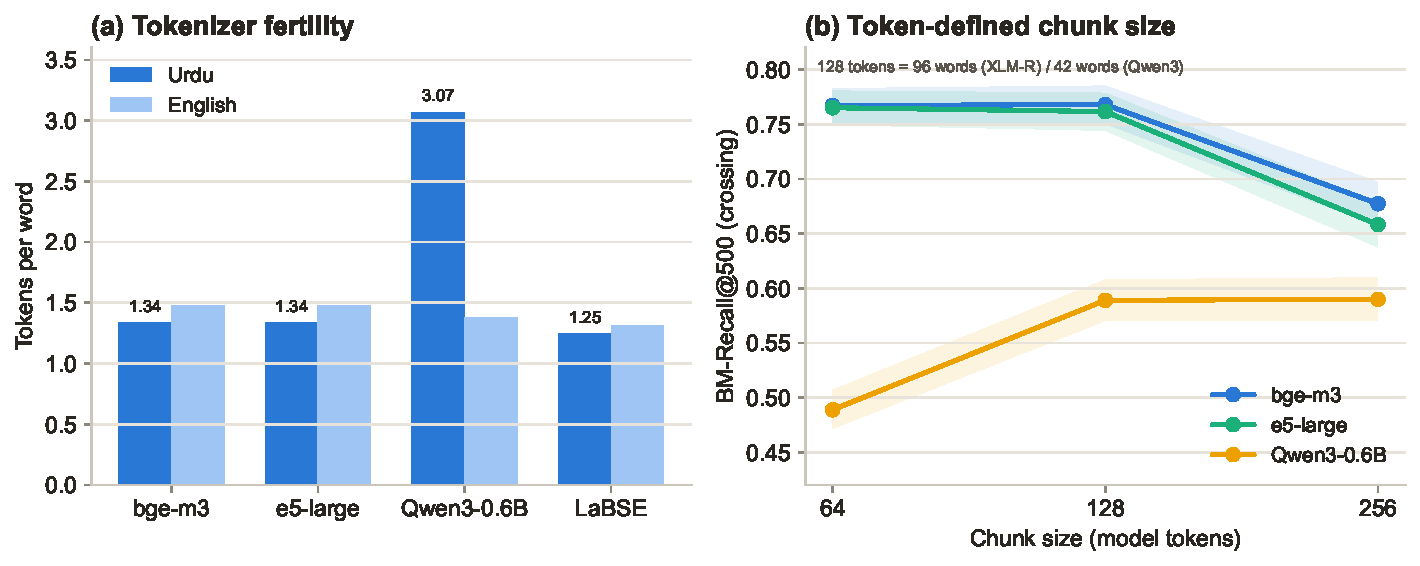
\includegraphics[width=0.92\textwidth]{../figures/fig2_token_units.pdf}
\caption{(a) Tokens per whitespace word by tokenizer. (b) BM-Recall@500 against token budget.
Bands are 95\% article-level bootstrap CIs. Adjacent token budgets are statistically tied;
the same budget is a different amount of text for each tokenizer.}
\label{fig:tokens}
\end{figure*}

\begin{table}[t]
\centering
\small
\begin{tabular}{lcccc}
\toprule
Model & 64 & 128 & 256 & words at argmax \\
\midrule
bge-m3 & .767 & \bb{.768} & .677 & 96 \\
e5-large & \bb{.765} & .762 & .658 & 48 \\
Qwen3-0.6B & .489 & .589 & \bb{.590} & 83 \\
\bottomrule
\end{tabular}
\caption{BM-Recall@500 by token budget (top row: tokens; bottom row: implied whitespace words at
the selected budget).}
\label{tab:tokens}
\end{table}

\subsection{Boundaries and normalization}
\label{sec:norm}

At 50 words, sentence-aware splitting beats the English recursive default in all four systems where
both were run (LaBSE was not run with recursive-English; Figure~\ref{fig:split}): bge-m3 +6.02
[4.98, 7.06], e5 +6.21 [5.18, 7.21], Qwen3 +6.90 [5.59, 8.15], BM25 +5.53 [4.31, 6.70]. Against fixed-size chunks the gain is larger: +11.4, +11.0, +12.7,
and +10.1 points. At 100 words it shrinks and turns mixed (bge +1.41 [0.30, 2.53]; e5 +0.86
[$-$0.32, 1.99]; Qwen3 $-$2.04 [$-3.34$, $-$0.74]). At 200 it reverses: bge $-$8.99, e5 $-$10.38,
Qwen3 $-$11.75, BM25 $-$3.09.

The answer-split rate shows part of the mechanism. Fixed 50-word chunks cut 4.10\% of answers;
sentence-aware 50-word chunks cut 0.05\%. At 200 words the rates are 1.06\% and 0.00\%. The reversal
is therefore not about splitting. The English recursive rule, applied to Urdu, produces smaller
units and a different retrieval granularity at large targets. This is an interaction, not a free win.

Normalization barely moves. N1 and N2 differ from N0 by at most 0.09 points. Every article-level CI
covers zero except a 0.085-point N2 gain for BM25 at 50 words ($p=0.038$, uncorrected and
exploratory). The Unicode audit
explains why: no ZWNJ or ZWJ, one tatweel, nine Arabic yeh characters, 34 Urdu digits. We
report the null instead of dressing it up.

\begin{figure}[t]
\centering
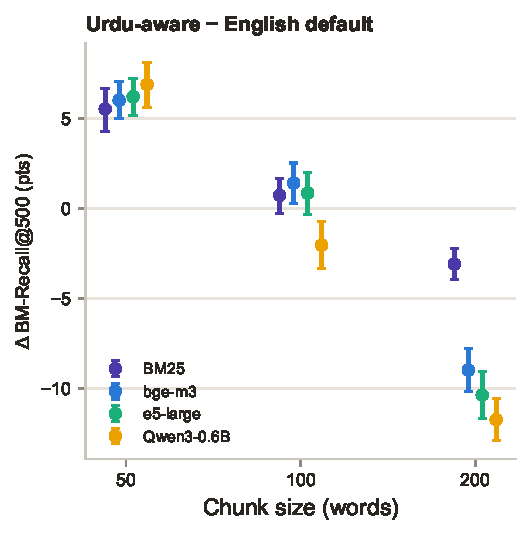
\includegraphics[width=\columnwidth]{../figures/fig3_urdu_vs_english_splitting.pdf}
\caption{Difference between Urdu-aware sentence splitting and the English recursive default
(bm500x, points). Positive means Urdu-aware is better. The advantage at 50 words reverses at 200.}
\label{fig:split}
\end{figure}

\subsection{Overlap}

Against the English studies we reviewed, 25\% overlap helps at every tested size in the four
systems where overlap was run (LaBSE was not; Figure~\ref{fig:overlap}). bge-m3 gains 6.91 [5.72, 8.05] at 50 words, 5.24 [4.29, 6.18] at 100,
and 4.22 [3.10, 5.38] at 200. e5 gains 7.16, 5.13, and 3.77; Qwen3 6.13, 5.75, and 4.97. BM25
follows with 6.97, 5.51, and 2.60. Overlap keeps spans intact and gives 50-word chunks enough
surrounding text to rank. Both effects are visible in the per-question data. The result is
corpus-specific; we do not claim it travels.

\begin{figure*}[t]
\centering
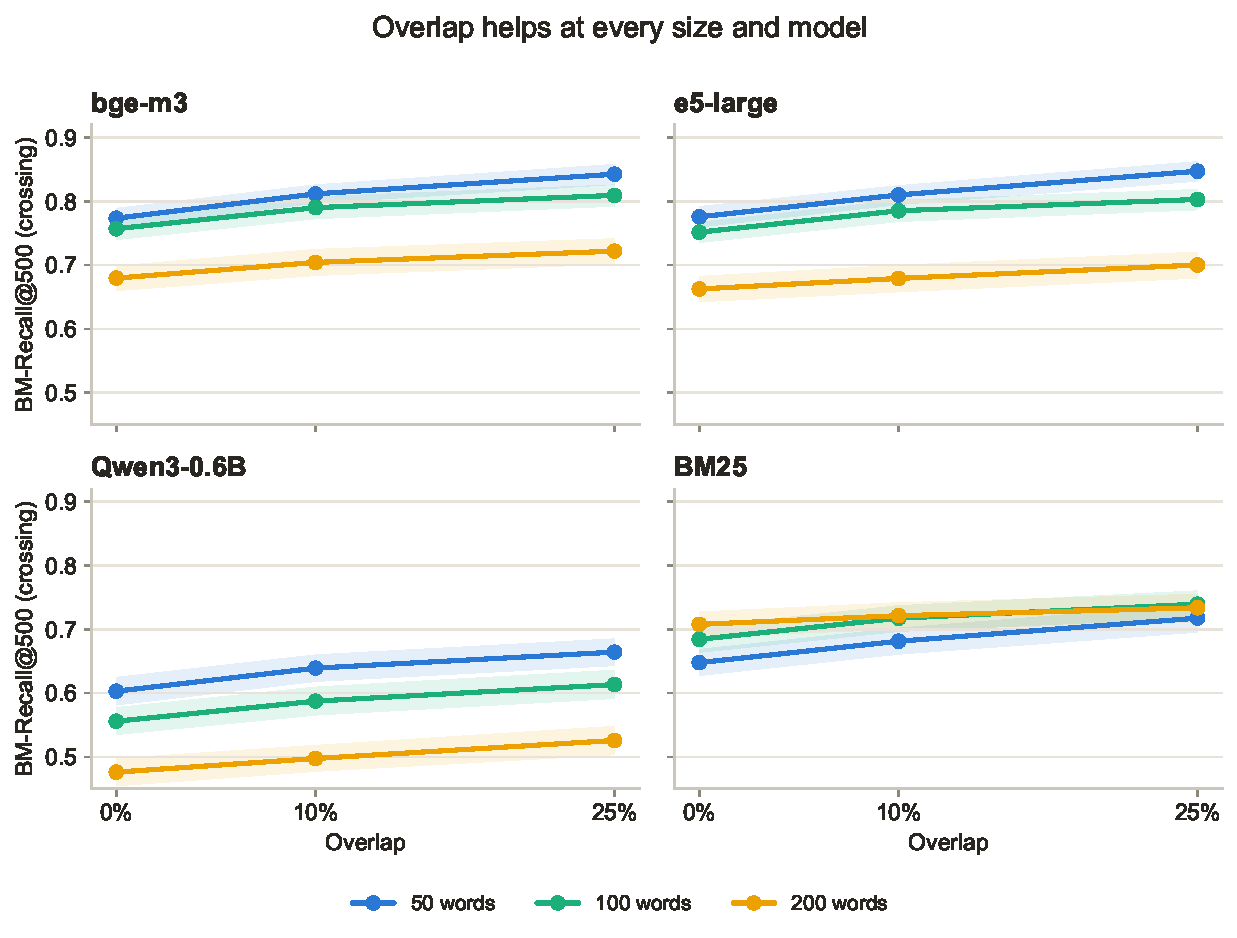
\includegraphics[width=0.84\textwidth]{../figures/fig4_overlap.pdf}
\caption{BM-Recall@500 against overlap for four systems and three sizes. Bands are 95\%
article-level bootstrap CIs. Overlap helps everywhere; the effect is largest at 50 words.}
\label{fig:overlap}
\end{figure*}

\subsection{English control}

English is easier on the parallel questions, but the best tested fixed-word size does not move:
50 words in both languages (Table~\ref{tab:english}). The gap is 7.4 points at 50, 7.2 at 100, and 7.8 at 200.
For recursive-English chunks it is 10.8 at 50, 6.3 at 100, and gone at 200 ($-$0.9 [$-2.29$,
0.46]). Nothing here says the languages need different sizes. It does say the Urdu side is harder,
which fits translation artifacts and weaker Urdu coverage in the encoders.

\begin{table}[t]
\centering
\small
\begin{tabular}{llccc}
\toprule
Strategy & Size & Urdu & English & Diff. \\
\midrule
fixed words & 50 & .773 & .847 & +7.4 \\
fixed words & 100 & .757 & .829 & +7.2 \\
fixed words & 200 & .680 & .758 & +7.8 \\
recursive English & 50 & .828 & .935 & +10.8 \\
recursive English & 100 & .836 & .899 & +6.3 \\
recursive English & 200 & .809 & .800 & $-$0.9 \\
\bottomrule
\end{tabular}
\caption{Parallel English control with bge-m3. Diff.\ is English minus Urdu in points; the 200-word
recursive difference is not significant.}
\label{tab:english}
\end{table}

\subsection{Best systems}

Sentence-aware 50-word chunks with bge-m3 score 0.888 [0.876, 0.899]. e5 is 0.886 [0.873, 0.897];
the two are tied. RRF reaches 0.871 [0.857, 0.884] with bge and 0.865 with e5, below the best single
model. It does lift the weak ones: Qwen3 from 0.730 to 0.814, LaBSE from 0.703 to 0.810, BM25 from
0.749 to 0.871. BM25-char trails BM25-whitespace by 2--4 points at every size. Table~\ref{tab:best}
has the full ranking.

\begin{table}[t]
\centering
\small
\begin{tabular}{lc}
\toprule
System & BM-Recall@500 \\
\midrule
bge-m3, sentence-aware 50 & \bb{.888} [.876, .899] \\
e5-large, sentence-aware 50 & .886 [.873, .897] \\
bge-m3 + RRF & .871 [.857, .884] \\
BM25, sentence-aware 50 & .749 [.728, .769] \\
Qwen3-0.6B, sentence-aware 50 & .730 [.710, .750] \\
LaBSE, sentence-aware 50 & .703 [.683, .723] \\
\bottomrule
\end{tabular}
\caption{Best configuration per system (95\% article-level bootstrap CIs).}
\label{tab:best}
\end{table}

\section{Discussion}

\paragraph{Words are the portable unit; tokens are not.}
Specify chunk size in words when encoders use different tokenizers. A word is a language unit. A
token is a model unit whose size depends on the vocabulary. The measured fertility gap here is
2.3$\times$ (1.34 vs.\ 3.07). That is enough to turn one nominal configuration into two different
retrieval tasks. The token argmaxes are plateaus, so the problem is not a sharp 64-versus-256
disagreement. It is that ``128 tokens'' does not name a fixed amount of text.

\paragraph{Boundary for three encoders; bge-m3 confirmed downward.}
Above 50 words every dense curve falls. For e5, Qwen3, and LaBSE, 50 is the smallest size tested.
For bge-m3, 10--50 are now tested and 50 is still best; the curve rises monotonically into 50. The
40- and 50-word intervals overlap, so the lower end is not sharply separated, and 30/35/45 remain
untested. The data show that the best \emph{tested} size is the same across encoders; they do not
show that 50 is optimal in any absolute sense. The boundary also explains why Urdu-aware splitting
gains most at 50 words: sentence-aware chunks avoid the 4.1\% answer-split rate of fixed 50-word
chunks.

\paragraph{Why overlap helps here.}
English chunking work often finds overlap neutral or harmful
\citep{bennani2026a,amiri2025chunk}. This corpus differs in two ways. Documents are concatenations
of short translated paragraphs, and answers are short spans. Overlap keeps a span intact when a
boundary would cut it, and it gives 50-word chunks context they otherwise lack. Four systems show
the same direction, so it is not one model's quirk. It remains a corpus-specific result.

\paragraph{Language-aware splitting is conditional.}
Urdu-aware splitting is not a free win. At 50 words it beats the English default by six points. At
200 words it loses 3 points for BM25 and 9--12 for the dense encoders. A paper that reported one
size could reach the opposite conclusion.
The Khmer result fits this pattern \citep{chhoun2026evaluation}: language-aware chunkers interact
with size and with the recursive merge policy. One size is not a test.

\paragraph{Normalization is a property of the corpus.}
The null is informative. UQA's translation pipeline already produces normalized Urdu: no ZWNJ,
essentially no tatweel, almost all digits ASCII (34 are Urdu digits), and nine Arabic-variant yeh characters. A study on
naturally occurring Urdu web text could still find an effect. Here there is almost nothing to
normalize. We report the Unicode audit so the null can be read rather than guessed at.

\section{Limitations}

\begin{itemize}
\item \bb{Machine-translated corpus.} UQA is MT, with 4.86 variants per paragraph. The modal rule
  keeps 20\% of rows and may select a systematically different translation. The English control is
  original SQuAD text, so the language comparison mixes language with translation artifacts.
\item \bb{Boundary result.} 50 words is the smallest size tested for e5, Qwen3, and LaBSE. bge-m3
  was extended to 10/25/40/50; 50 remains best and the curve is monotonic, but 30/35/45 are untested
  and no interior maximum is identified.
\item \bb{Single domain.} Wikipedia articles made of concatenated paragraphs. Not web text, legal
  text, or conversation.
\item \bb{Machine-translated queries.} Every question is UQA machine translation. The 150--300
  native-authored questions needed to test transfer do not exist. Three raters judge 77 of 100
  sampled questions self-contained by majority (Wilson 95\% CI 67.8--84.2\%; Fleiss' kappa 0.734);
  one row is unclear and one has no majority.
\item \bb{Retrieval only.} No generator and no LLM judge. The conclusions concern evidence
  retrieval, not answer quality. Relevance is exact answer-string containment; no human relevance
  or context-quality judgments were collected.
\item \bb{Selection and multiplicity.} Confidence intervals are marginal, not adjusted for the many
  configurations, and the best system in Table~\ref{tab:best} was selected after inspecting all
  runs; its interval is optimistically narrow. The one $p=0.038$ normalization contrast would not
  survive a strict multiplicity correction.
\item \bb{Fixed BM25.} $k_1$ and $b$ were fixed in advance, not tuned. A tuned BM25 is a different
  experiment.
\item \bb{Small normalization exclusions.} 37 of 9{,}077 questions (0.41\%) fail N1/N2 span
  mapping because UQA answers are whitespace-padded. They are excluded from those variants only.
\item \bb{Prefix sensitivity.} Qwen3's documented instruction prefix lowered BM500 relative to no
  prefix (0.400 vs.\ 0.460). Its absolute numbers may understate the model.
\end{itemize}

\section{Ethics and Reproducibility}

SQuAD2.0 is CC BY-SA 4.0. UQA has no explicit licence, so the public artifact contains code,
configurations, question IDs, and per-question metrics rather than UQA text. It is available at the
public repository:
\begin{flushleft}\footnotesize\href{https://github.com/devxyasir/urdu-chunking-strategy}{github.com/devxyasir/urdu-chunking-strategy}\end{flushleft}
The corpus is encyclopedic and contains no personal or sensitive data. No LLM generated evaluation data, labels, or rankings. Every question
and span comes from the released corpora, and every metric is deterministic. We report 360 main
runs and 4 lower-size runs, bootstrap seed 0, model revisions, per-question metrics, and
article-level CIs. AI assistance was
used for literature search, code development, analysis, figure generation, and drafting/editing.
The author verified all results and takes responsibility for the content.

\section{Conclusion}

For Urdu retrieval, define chunk size in words, not model tokens. The same token budget is 96 words
for XLM-R and 42 for Qwen3, while the best tested word size is 50 for every encoder; extending
bge-m3 down to 10 words does not move it. Urdu-aware sentence splitting helps at the sizes dense
retrievers prefer (5.5--6.9 points) and reverses at 200 words. 25\% overlap helps on this corpus. Normalization is a null on machine-translated Urdu. We
release the pipeline and per-question results so the size-by-unit interaction can be tested on
other languages and on naturally occurring text.

\bibliography{refs}

\appendix
\section{Additional results}

\paragraph{Strict versus crossing budget.}
The main text uses the crossing definition. Under the strict definition the BM25 argmax moves from
200 to 100 words (0.686 at 100, 0.663 at 200). Every dense argmax stays at 50. No dense conclusion
changes.

\paragraph{Normalization.}
N0/N1/N2 means for BM25-whitespace at 50/100/200 words differ by at most 0.09 points. The largest
difference is N2 at 50 words (+0.085, $p=0.038$, uncorrected and exploratory). N1/N2 exclude 37
whitespace-padded answers.

\paragraph{Prefix checks.}
On 100 dev questions at 200 words, the e5 instruction prefix improves BM500 from 0.550 to 0.640 and
R@1 from 0.43 to 0.49. The Qwen3 prefix changes BM500 from 0.460 to 0.400 and R@1 from 0.31 to 0.32.
Both models use their documented format in every reported run.

\paragraph{Grid.}
BM25: 2 sparse variants $\times$ (75 base configurations + 6 N1/N2 normalization runs) = 162 runs.
Dense: 54 for bge-m3 (21 Urdu + 12 at 400/800 + 21 English), 21 for e5, 33 for Qwen3
(21 + 12 at 400/800), and 6 for LaBSE = 114 runs. RRF: 84 runs. Total 162 + 114 + 84 = 360.
The 21-configuration base is fixed words at 50/100/200 with 0/10/25\% overlap (9), fixed tokens at
64/128/256 (3), and sentence-aware, recursive-English, and recursive-Urdu at 50/100/200 with zero
overlap (9). The lower-size check adds 4 bge-m3 runs at 10/25/40/50 words (zero overlap, N0), for
364 runs including the extension. The check is reported separately in \S\ref{sec:lower}; it is not
part of the archived 360-run package.

\paragraph{Model revisions and environment.}
\begin{flushleft}\footnotesize
Model revisions: bge-m3 \textsf{5617a9f61b028005a4858fdac845db406aefb181}\\
e5 \textsf{274baa43b0e13e37fafa6428dbc7938e62e5c439}\\
Qwen3 \textsf{97b0c614be4d77ee51c0cef4e5f07c00f9eb65b3}\\
LaBSE \textsf{836121a0533e5664b21c7aacc5d22951f2b8b25b}
\end{flushleft}
The archived runs used sentence-transformers
6.2.0, transformers 5.20.2, torch 2.11.0+cu130, CUDA 13.0, and one NVIDIA A100-SXM4-40GB. The
bootstrap uses seed 0. The manifest's \textsf{budget\_mode\_primary} key records a hard-coded label
from an earlier draft; the primary metric in every table is \textsf{bm500x} (crossing), and
\textsf{bm500} is the strict variant.

\end{document}
